\section{Simulation tools}

Several simulation tools were used in CLAS12 Trigger System Project. Those tools were very useful during development stage and still in use now for validation.


\subsection{GEMC/GEANT4 simulation tool}

In the beginning of the CLAS12 trigger system development hardware was not available, so input data were generated by Geant4 Monte-Carlo package (GEMC, \ref). That package was used to produce data files with data banks in the same form it will be produced by DAQ. Trigger system software includes playback package which is able to read GEMC-generated files and produce FADC and DCRB responce identical to the one from real hardware. All Stage 1 trigger components implemented with HLS were developed using simulated data, including most complex ones in calorimeter and drift chamber. For VHDL-written components simulated data were used as well along with other specialized tools described below.

For example Fig.~\ref{fig:ecal_sim1} and Fig.~\ref{fig:ecal_sim2} shows the comparison of the energy and coordinates of the EC clusters reconstructed by offline analysis software and by trigger system. Different dividers were used in trigger system: DSP-based one in first case and lookup table-based in second one. First method provides better results but requires more resources that second one. Over the course of system development many decisions were made based on similar comparisions.

\begin{figure}[htp]
	\begin{center}
		\centering
		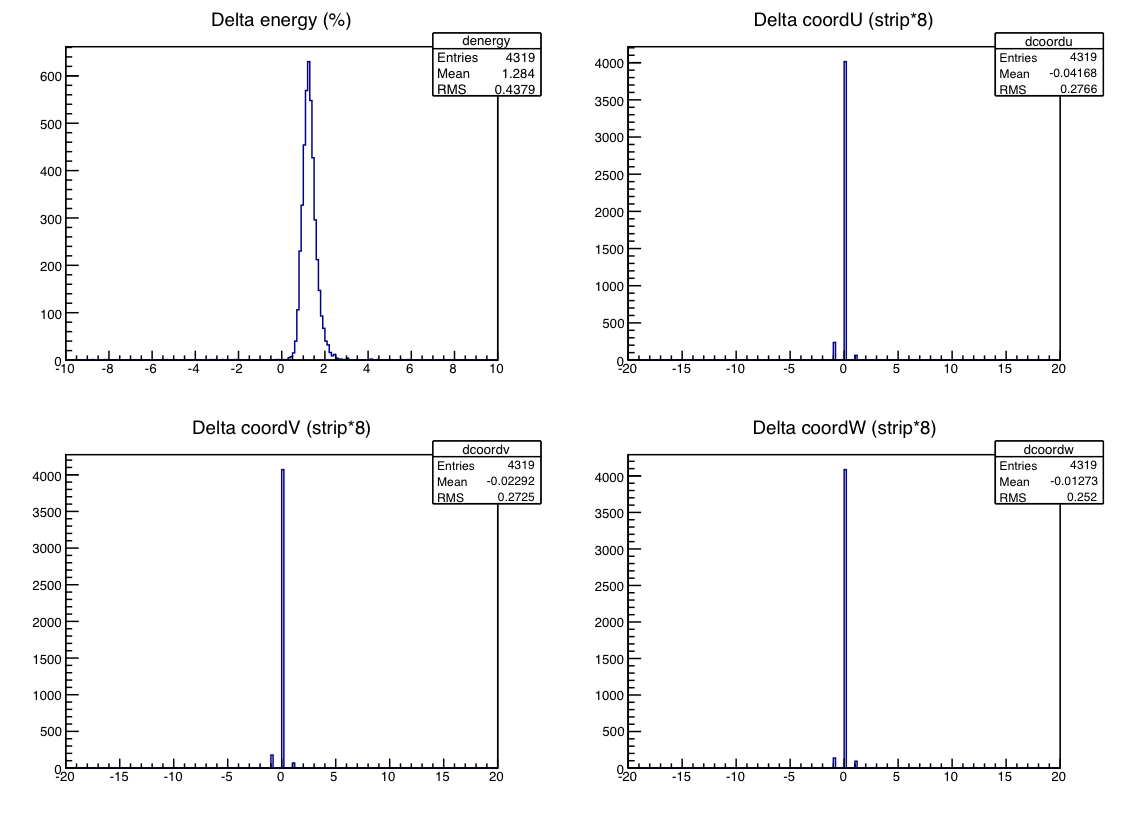
\includegraphics[width=8cm]{img/ecal_sim1.png}
		\caption{EC cluster finding: difference between results from offline reconstruction and trigger system (using dividing in coordinate calculation)}
		\label{fig:ecal_sim1}
	\end{center}
\end{figure} 

\begin{figure}[htp]
	\begin{center}
		\centering
		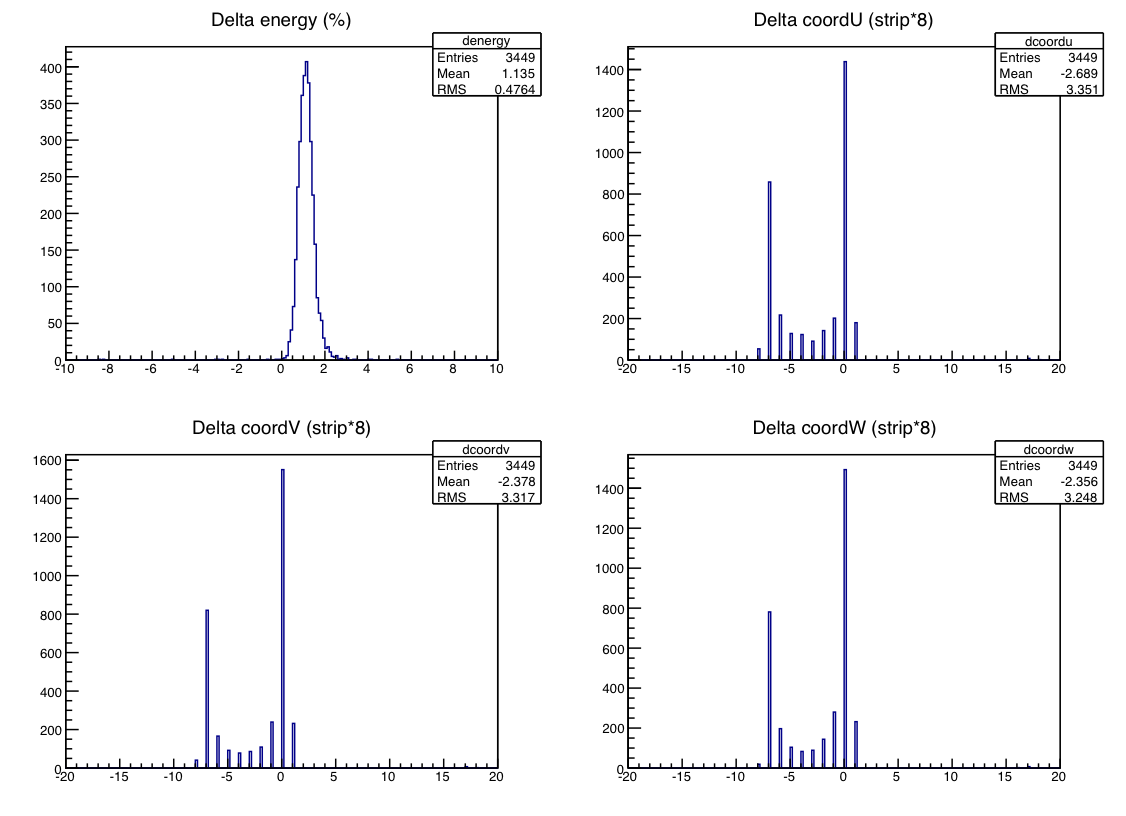
\includegraphics[width=8cm]{img/ecal_sim2.png}
		\caption{EC cluster finding: difference between results from offline reconstruction and trigger system (using lookup table in coordinate calculation)}
		\label{fig:ecal_sim2}
	\end{center}
\end{figure} 

Another example Fig.~\ref{fig:ecal_sim3} shows absolute cluster energy obtained by offline analysis and by trigger system. As it can be seen trigger system provides the same result as predicted by simulation and obtained from offlne analysis.

\begin{figure}[htp]
	\begin{center}
		\centering
		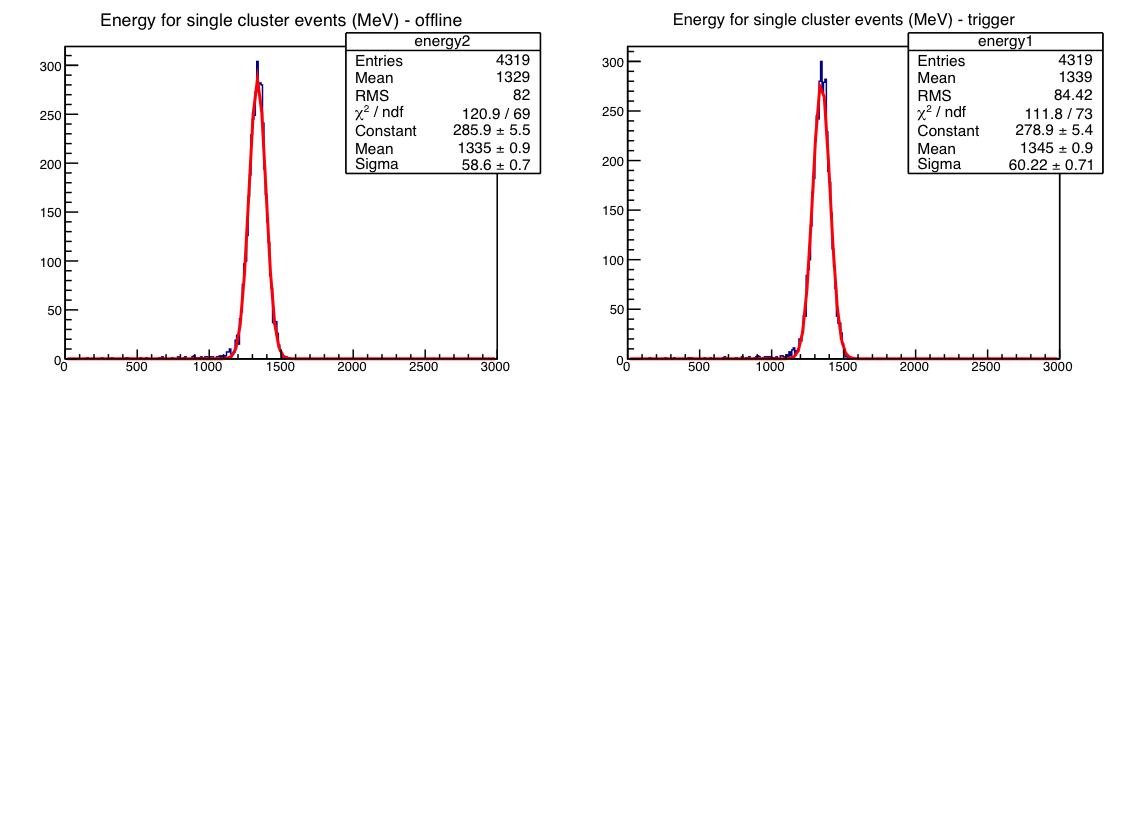
\includegraphics[width=8cm]{img/ecal_sim3.png}
		\caption{EC cluster finding: 5GeV electron, no PCAL, energy deposition in offline and trigger model}
		\label{fig:ecal_sim3}
	\end{center}
\end{figure} 


\subsection{FPGA simulation tools}

A cycle accurate simulator was setup to model, test, and debug the full trigger system using Aldec Riviera. This tool is able to perform simulations of the full trigger system in a mixed language environment (VHDL, Verilog, C/C++) for all FPGA components used in CLAS12 (Xilinx series 5, 6,and 7 components). VHPI was used to interface external C/C++ programs from the DAQ to the VHDL testbench. Using VHPI, calls to the DAQ EVIO C/C++ libraries were possible from VHDL making it possible to feed detector waveform data into the trigger simulation directly from Monte-Carlo, data files taken with beam, or from user created text files. Simulation intensive components, primarily gigabit SerDes components, were replaced with fast, simple models once verified to improve the simulation performance. The simulator is single-threaded and requires a license for each running instance, making it costly to parallelize. Even so, it was capable processing 1 event every ~30 seconds on a typical desktop PC simulating the forward and central trigger system comprised of 24,192 drift chamber wires and ~3400 FADC250 channels.

The simulation was built from the actual firmware HDL firmware source files compiled for the various modules used in the trigger system (DCRB, FADC250, VTP, SSP). HDL wrappers were created to model the VXS crates which includes: backplane, fiber interconnect, trigger distribution, clock distribution, configuration, and readout. The following table summarizes the trigger simulation components:

\begin{center}
	Trigger Simulation crates\\
	\begin{tabular}{| l | l | l | l | l |}
		\hline \hline
		System		& Crates	& ModType	& ModCnt	& ChCnt		\\
		\hline
		DC		& 18		& DCRB		& 252		& 24192		\\
		ECAL		& 6		& FADC250	& 84		& 1296	 	\\
		PCAL		& 6		& FADC250	& 96		& 1152	 	\\
		FTOF		& 6		& FADC250	& 36		& 576	 	\\
		FTCAL		& 2		& FADC250	& 21		& 332	 	\\
		FTHODO		& 1		& FADC250	& 15		& 232	 	\\
		CND		& 1		& FADC250	& 9		& 144	 	\\
		CTOF		& 1		& FADC250	& 6		& 96	 	\\
		HTCC		& 1		& FADC250	& 3		& 48	 	\\
		GT		& 1		& SSP		& 6		& 28 (Fiber)	\\
		\hline \hline
	\end{tabular}
\end{center}

Each of the front-end crates use a VTP trigger module that run the detector specific trigger algorithm. The front-end VTP modules fed trigger data to the global trigger (GT) crate stage 2 (SSP). The SSP modules fed trigger data into the final trigger stage 3 (GTP). There are 10 different VTP firmware types to support the stage 1 (front-end) and stage 3 (GTP) algorithm. There are 2 different SSP firmware types that support the stage 2 forward and central detector trigger logic.

This full simulation is primarily run for two scenarios. First is when a significant firmware change is made a small number of specially selected events (~2k) can be fed through to tag the trigger decisions on each. Second is when the real DAQ system records events where the trigger failed to properly tag them (typically during a random trigger run to assess the efficiency). For both cases the failed events can be loaded into the simulation and failed decisions explored in detail to determine the cause. The first scenario takes ~1 day or more depending on the number of events needed to check, while the second case can take minutes since only failed events are presented to the simulation so problems can immediately begin to be examined.